\documentclass[a4paper,11pt,reqno]{amsart}

\pagestyle{headings}
\usepackage{graphicx}
\usepackage[english]{babel}
\usepackage[T1]{fontenc}
\usepackage[latin1]{inputenc}
\usepackage{verbatim}
\usepackage{amsmath}
\usepackage{amsfonts}
\usepackage{amssymb}
\usepackage{amsthm}
\usepackage{pstricks}
\usepackage{mathrsfs}
\usepackage{textcomp}
\usepackage{tikz}
\usepackage{subfig}

\title{Bare-metal programming on the Raspberry Pi 2}
\author{Didrik Lundberg\\
\texttt{didrikl@kth.se}}
\date{\today}
\begin{document}
\maketitle
\noindent
This is a comprehensive guide that will cover all steps of bare-metal programming necessary to run the SICS Thin Hypervisor for the Raspberry Pi 2. If you have any questions, please send an E-mail to the author.
\section{Introduction}
In order to follow this guide, you will need some equipment:
\begin{itemize}
  \item A Raspberry Pi 2 Model B single-board computer
  \item A PC to program on
  \item Internet connection via an Ethernet cable
  \item An SD card reader
  \item A serial-to-USB converter cable
  \item A USB to serial interface converter module (for JTAG)
  \item For testing the hardware:
  \begin{itemize}
    \item A USB mouse and a USB keyboard
    \item A monitor with a HDMI cable connection
  \end{itemize}
\end{itemize}
The four first items should be pretty straightforward to acquire. RPi2 uses micro-SD cards, so you will require your SD card reader to be able to read those. The serial port of the RPi2 is more specifically a UART using the 3.3V TTL standard of voltages - please note that converter cables which use other standards, such as RS-232, may fry your RPi2! However, some cables work for both RS-232 and 3.3V TTL. Look up the specifications of the chip in the converter cable you are buying just to be sure.

The UART communicates via two GPIO pins on the ordinary RPi2 pin block. However, the serial-to-USB converter cable should typically have four jumper wire connectors on one end and a USB connector on the other (the two additional wires providing ground and 5V power). If you find this to be confusing to sort it out yourself, I bought a serial-to-USB converter cable which uses the PL2303HX chip to transform the signal which I recommend - that chip name might be a good word to search the Internet for if you want to buy one yourself.

\section{Testing the equipment}
First, we must make sure that all our equipment is functional. To do this, we first download NOOBS from the homepage of the Raspberry Foundation. NOOBS is an operating systems installer, which we will use to comfortably set up Raspbian for testing purposes.

Simply format your SD card in the FAT32 file system (using for example \texttt{gparted}) and transfer the decompressed contents of the NOOBS folder to it, and you are ready to boot your RPi2 for the first time. Put your SD card in the RPi2, connect the Ethernet cable, the USB keyboard and mouse, the monitor, and then finally plug in the micro-USB cable (connected to your PC or to a USB power adapter of good quality on the other end) to supply power and your RPi2 will boot into NOOBS.

Install Raspbian, and inside Raspbian install the \texttt{screen} utility by typing \texttt{sudo apt-get install screen} in the terminal. Also install \texttt{screen} on the PC you are programming on.

Now it is time to connect the RPi2 to your computer with serial-to-USB converter cable. You must do this with great care, since connecting the wrong jumper wire to certain pins might fry your RPi2. We will explain how to do this for our generic PL2303HX cable. It has four jumper wires:

\begin{itemize}
  \item \textbf{TxD}: Green. The ``T'' in the acronym stands for ``transmission'' - should be connected to the UART receiver pin (RxD) on the RPi2 block.
  \item \textbf{RxD}: White. The ``R'' in the acronym stands for ``receiving'' - should be connected to the UART transmission pin (TxD) on the RPi2 block.
  \item \textbf{Ground}: Black. Should be connected to the Ground pin on the RPi2 pin block.
  \item \textbf{5V power}: Red. WARNING! Do not plug this cable in if you are also supplying power via a micro-USB cable - that might fry the RPi2. This cable is an alternate way of providing power to the RPi2 without using a micro-USB cable.
\end{itemize}

It is important to note that the pin layout of the RPi2 is closely resembles that of other versions, the difference being that it has more pins (40 compared to 26 for the RPi). The 26 first pins counting from the pin closest to the SD card have the same functions. There are two ways of numbering the GPIO pins - using their GPIO numbers by which they are referred to by the computer, or using how they are physically ordered on the board, which might be a source of some confusion.
\begin{figure}[hb]
\begin{center}
   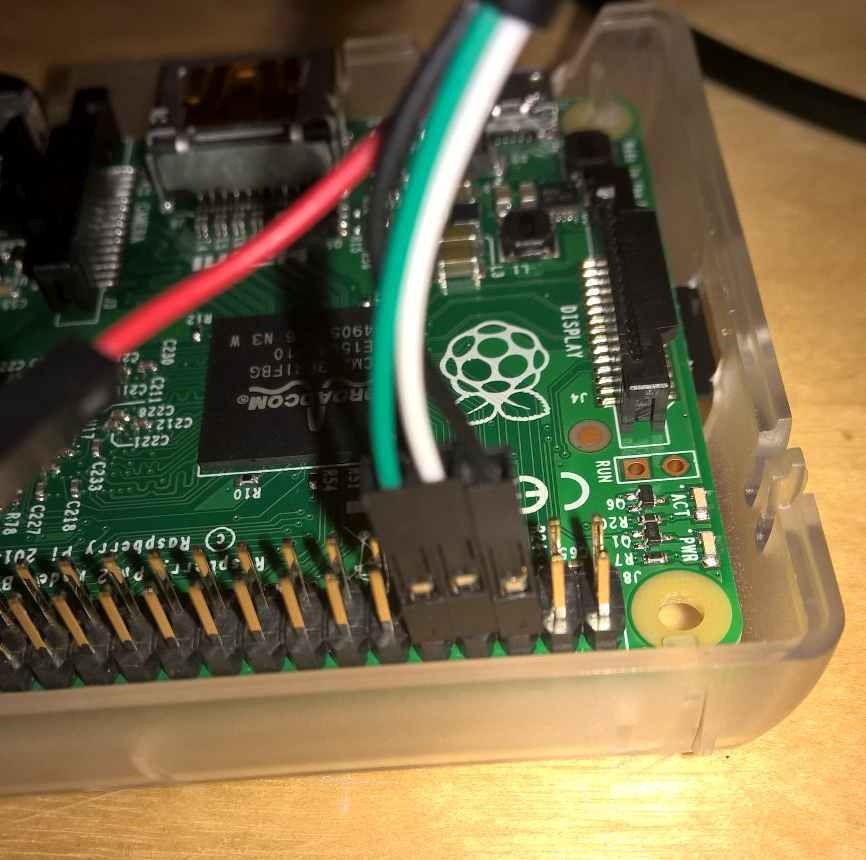
\includegraphics[scale=0.3]{connection.png}
 \end{center}
 \caption{The serial-to-USB converter as it looks connected to the RPi2}
 \label{fig:conn}
\end{figure}
\begin{figure}[hb]
\begin{center}
   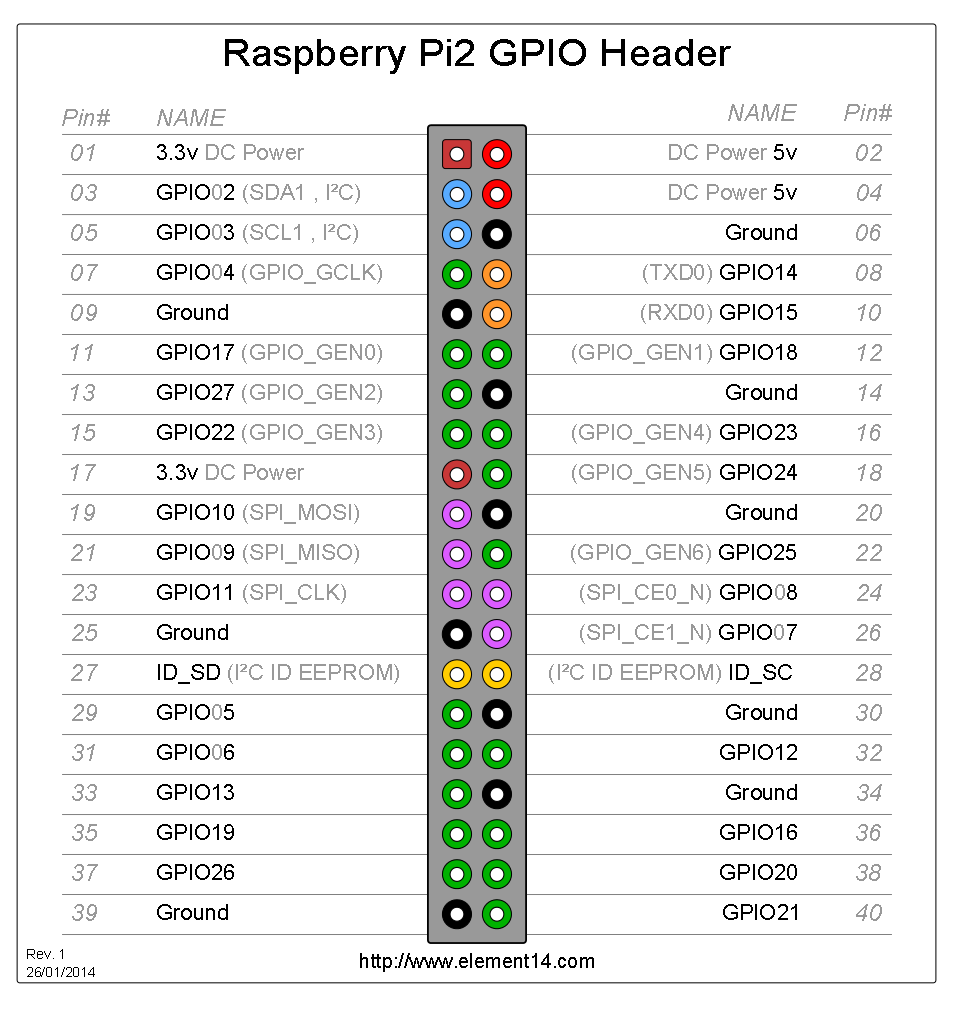
\includegraphics[scale=0.3]{GPIO_Pi2.png}
 \end{center}
 \caption{The RPi2 pin numbering}
 \label{fig:pins}
\end{figure}

So, by the above physical numbering seen in Figure~\ref{fig:pins}, the ground wire should be connected to pin 6, the receieve wire should be connected to pin 8, and the transmit wire to pin 10, as shown in Figure~\ref{fig:conn}. If you know what you are doing, you can also power the RPi2 by connecting the power wire to pin 2 or 4, but then you risk frying your equipment if you supply power over the micro-USB at the same time, so I would not recommend this.

Now, you first want to check that the serial-to-USB cable works correctly. To do this, write \texttt{lsusb} in a terminal window, and you should see a list of connected USB devices, in which the serial-to-USB cable should be identified. Second, we need to know the device name of the cable. Simply use \texttt{dmesg | grep usb} and you should be able to filter out the device name of the cable among the driver messages (in my case \texttt{/dev/ttyUSB0}).

Setting up the connection on the RPi2 should be easy - simply write \texttt{sudo screen /dev/ttyAMA0 115200}. The number at the end is the symbol rate of the connection, measured in bauds (bits per second). Similarly, on your computer, write \texttt{sudo screen /dev/ttyUSB0 115200}, where you replace the device name if needed. Now, if everything works correctly you should be able to write on the PC and see the characters appearing on the monitor connected to the RPi2, and vice versa. This ensures us that all the hardware works correctly, saving us valuable time looking for errors later if that should not be the case.

\section{Writing a test program}
Now, you will need an empty SD card. Either re-format the one you have, again to FAT-32, or use another one, which might be more handy if you need Raspbian later on.

Writing a bare-metal program requires intimate knowledge about the hardware. The hardware of the RPi2 is very similar to that of the RPi, whose chip BCM2835 has excellent documentation. The only significant difference is the processor, and the increased RAM of the RPi2. Indeed, there are more differences, such as for example a mini-UART which is not on the RPi2, but these differences are not relevant for this guide.

It follows that we can use the BCM2835 documentation for working with the RPi2, with a few important corrections: the base address of the peripherals has changed from \texttt{0x20000000} to \texttt{0x3F000000}, and the memory bus address offset \texttt{0x40000000} has changed to \texttt{0xC0000000}. Accordingly, all addresses you read in the documentation will have to be adjusted with this in mind. Typically, this just means that you replace \texttt{20} at the start of a hexadecimal number with \texttt{3F}.

Technically speaking, we are going to write a kernel -  although our ``kernel'' will not have much of the functionality we associate with one, it will take the place of a kernel during the boot process. It follows that we require a bootloader and other accessories to get running. The easiest way to solve this is to obtain the GitHub repository \texttt{raspberrypi/firmware} and copy the contents of the \texttt{boot} folder to your SD card, deleting the files \texttt{kernel.img} and \texttt{kernel7.img} (which are the existing kernels). We end up with some redundant files, but are guaranteed things will work.

\subsection{Setting up a cross-compiler}
You will require a compiler which can compile code to run on other hardware. This is easily solved by the GNU ARM Embedded Toolchain, which is installed by the command \texttt{sudo apt-get install gcc-arm-none-eabi} and you are good to go. Then, to compile \texttt{test.c}, you would use \texttt{arm-none-eabi-gcc -O2 -mfpu=vfp -mfloat-abi=hard -march=armv7-a -mtune=cortex-a7 -nostartfiles test.c -o kernel.elf}. However, we do not want an ELF file, but a binary which only includes machine code, so we extract that part from \texttt{kernel.elf} using the \texttt{objcopy} utility: \texttt{arm-none-eabi-objcopy kernel.elf -O binary kernel.img}, and get the binary we want in \texttt{kernel.img}. This can then be put on the SD card together with the bootloader, as described above, which will look for the kernel.img and execute it.

\subsection{Setting up CMake}
However, in reality we never just compile a single C file. We are going to have multiple files in C and ARM assembly language, and so we will need firstly a linker script and secondly CMake, in order to keep things neat.

\subsection{Example code}
Two useful example programs (or ``test kernels'') can be found in the GitHub repository \texttt{guancio/kth-on-rpi2}, in the \texttt{rpi2-port} folder.

\subsubsection{test-kernel-1}
This test kernel will make the green LED on the RPi2 blink, with approximately one-second intervals between each flash. This simple program is good for testing if your pipeline to get code running on the RPi2 is working correctly.

\subsubsection{test-kernel-2}
This test kernel will infinitely write alternately ``Hello, Kernel World!'' and ``Goodbye, Kernel World!'' over the UART, with approximately one second of waiting in between each output. This is useful for testing the serial connection.

\section{Booting over a network}
Start by downloading the GitHub repository \texttt{raspberrypi/firmware} (if you do not already have it downloaded) and copy the contents of the \texttt{boot} folder to your SD card, as described before. Then, open the file \texttt{config.txt} on your SD card, and change it to read \texttt{kernel=u-boot.bin}, instead of where \texttt{kernel} pointed to before.

Next, you will need to create a script that U-Boot will run once it is started. Create a file called \texttt{boot.scr}, and enter the following:

\begin{verbatim}
usb start
setenv scriptaddr 0x02000000
setenv serverip 130.229.149.236
setenv ipaddr 130.237.224.169
setenv bootargs "console=tty0"
tftp ${kernel_addr_r} zImage
bootz ${kernel_addr_r}
\end{verbatim}

where you replace the IP address after \texttt{serverip} by the one of your computer (which will act as a TFTP server later on). Your IP address can be found by looking at your \texttt{inet addr} after executing the \texttt{ifconfig} command in a terminal window.

Also replace the IP address after \texttt{ipaddr} in the boot script by an address belonging to your local network which is currently unoccupied - this will be the IP address of the RPi2. As a strategy, choose an address close to yours (alter only numbers near the right end of the IP) and ping it, using the command \texttt{ping 130.237.224.169}, where you replace the IP address with the one you want as the IP address of your device.

It might also be worth noting that \texttt{usb start} scans bus 0 for storage and Ethernet devices, which include your Ethernet port. Without this line, you will not be able to connect to your computer via TFTP. The \texttt{scriptaddr} is explicitly defined in the script for pedagogic reasons. This might not be needed, but you need to remember to not overwrite U-Boot on memory with the boot script. 

This bootscript presupposes that you have a monitor connected to the RPi2 via a HDMI cable. If you instead rely on serial connection to see what is happening (not recommended at this point), you should replace \texttt{console=tty0} with \texttt{console=ttyAMA0} (or simply use both). Bootargs usually also sets properties of the file system, but since we are not using it in our trivial examples, it is not needed here.

Now that we have written the bootscript, we want to convert it to an image. Do this by executing the command \texttt{mkimage -A arm -O linux -T script -C none -n Boot Script -d boot.scr boot.scr.uimg}. The result will be stored in \texttt{boot.scr.uimg} - transfer this file to your SD card.

Now we only have one part left - U-Boot itself. First, we have to download U-Boot. Download it by executing the command \texttt{git clone git://git.denx.de/u-boot.git
}, which will create U-Boot to a directory at your current location. After that is done, we get the required cross-compiler by \texttt{apt-get install gcc-arm-linux-gnueabihf}. Also install U-Boot tools with \texttt{apt-get install u-boot-tools}. Now open a terminal window in the folder you have U-Boot in, and execute the command \texttt{make rpi\_2\_defconfig}, followed by \texttt{make all -j8}. After the build is finished, copy all files starting with \texttt{u-boot} to your SD card. Now, you can eject your SD card and place it in your RPi2.

We are now going to set up your computer as a TFTP server. First, we install the required tools by executing the command \texttt{sudo apt-get install xinetd tftpd tftp}. Edit (or create, if it does not exist) \texttt{tftp} in \texttt{etc/xinet.d/}, which should contain the following:
\begin{verbatim}
service tftp
{
	protocol        = udp
	port            = 69
	socket_type     = dgram
	wait            = yes
	user            = nobody
	server          = /usr/sbin/in.tftpd
	server_args     = /tftpboot
	disable         = no
}
\end{verbatim}

Then, create a directory called \texttt{tftpboot} in \texttt{/}. Make sure you do not have too stingy access rights by executing the commands \texttt{sudo chmod -R 777 /tftpboot} and \texttt{sudo chown -R nobody /tftpboot} in the directory where you created \texttt{tftpboot}. Then, make your changes take effect by executing \texttt{sudo service xinetd restart}.

Now, we need to prepare the kernel in question we want to remote boot. The boot script requires us to trick bootz into believeing it has received a Linux kernel. To do this, we must insert a so-called ``magic number'' \texttt{0x016F2818} into the code. Here, you will need a hex editor to verify what you are doing. Get one with the command \texttt{sudo apt-get install bless}. Enter the \texttt{boot.S} (or whatever the ARM assembler part of your kernel is named) and declare a dummy variable (with no name) by inserting the line \texttt{.word 0x016f2818} outside of a function. Compile the kernel, and then search for ``18286F01'' in the image file (not the ELF file) using the hex editor. These bytes should be found starting at the offset \texttt{0x24}. If they are at a higher offset in the program, move the declaration up in the \texttt{boot.S} file. If the bytes are found at a too low offset, declare more dummy variables (\texttt{.word 0x01010101}, and so on...) before the magic number until you can find it at the correct offset. Finally, when this is done, rename your kernel \texttt{zImage} and move it to the \texttt{tftpboot} directory.

The setup is now complete. Plug in an Ethernet cable and a HDMI cable connected to a monitor to your RPi2 and power it from micro-USB to observe your program booting from U-Boot.

If at any point you should shut down your computer, you will need to start the server again by writing \texttt{sudo /etc/init.d/xinetd restart}, and take a second look if the IP addresses in your boot script can still be used; otherwise you will need to change the bootscript, create the boot script image again, and transfer it to the SD card.

\section{Setting up JTAG}
TODO

\section{Changes to the hypervisor}
TODO

\end{document}
